\documentclass{article}
\usepackage[francais]{babel}
\usepackage[utf8]{inputenc} % Required for including letters with accents
\usepackage[T1]{fontenc} % Use 8-bit encoding that has 256 glyphs
\usepackage{pythontex}
\usepackage{amsthm}
\usepackage{amsmath}
\usepackage{amssymb}
\usepackage{mathrsfs}
\usepackage{graphicx}
\usepackage{geometry}
\usepackage{stmaryrd}
\usepackage{tikz}
\usetikzlibrary{patterns}
%\usetikzlibrary{intersections}
\usepackage[cache=false]{minted}

\usepackage{stmaryrd}
%\usepackage{tikz}
%\usetikzlibrary{tikzmark}
\usepackage{empheq}
\usepackage{longtable}
\usepackage{booktabs} 
\usepackage{array}
\usepackage{pstricks}
\usepackage{pst-3dplot}
\usepackage{pst-tree}
\usepackage{pstricks-add}
\usepackage{upgreek}
\definecolor{LightGray}{gray}{0.9}
\usepackage{eolgrab}
\usepackage{chngpage}
 \usepackage{calrsfs}
 % Appel du package pythontex 
\usepackage{pythontex}

\usepackage{algorithm2e}
\RestyleAlgo{algoruled}
  \SetKw{KwFrom}{from} 
\newenvironment{algo}{
\begin{algorithm}[H]
\DontPrintSemicolon \SetAlgoVlined}
{\end{algorithm}}



\usetikzlibrary{decorations.pathmorphing}
\def \de {{\rm d}}
\usepackage{color}
\usepackage{xcolor}
\newcommand{\mybox}[1]{\fbox{$\displaystyle#1$}}
\newcommand{\myredbox}[1]{\fcolorbox{red}{white}{$\displaystyle#1$}}
\newcommand{\mydoublebox}[1]{\fbox{\fbox{$\displaystyle#1$}}}
\newcommand{\myreddoublebox}[1]{\fcolorbox{red}{white}{\fcolorbox{red}{white}{$\displaystyle#1$}}}

\usepackage{xcolor}
%\setbeamercolor{background canvas}{bg=lightgray}
\usepackage{listings}
\definecolor{purple2}{RGB}{153,0,153} % there’s actually no standard purple
\definecolor{green2}{RGB}{0,153,0} % a
\lstset{%
language=Python, % 
basicstyle=\normalsize\ttfamily, % 
% Color settings to match IDLE style 
keywordstyle=\color{orange}, % 
keywordstyle={[2]\color{purple2}}, % 
stringstyle=\color{green2}, 
commentstyle=\color{red}, 
upquote=true, %
}
\lstdefinestyle{Python}{
    language        = Python,
    basicstyle      = \ttfamily,
    keywordstyle    = \color{blue},
    keywordstyle    = [2] \color{teal}, % just to check that it works
    stringstyle     = \color{violet},
    commentstyle    = \color{red}\ttfamily
}
 \title{Introduction à Git}
\author{Ibrahim ALAME}
\date{14/02/2023}
\begin{document}
\maketitle

\section{Qu'est ce qu'un système de contrôle de version ?}  
\subsection{Le problème du contrôle des versions}
Imaginez que vous avez un projet et que vous voulez créer une sauvegarde avant de faire des modifications qui sont susceptibles de rendre le projet non fonctionnel. Avant les logiciels de contrôle de version, la seule méthode était de créer un dossier pour votre sauvegarde, par exemple {\color{blue} v1.2}, puis de copier tous les fichiers dedans.

Mais les difficultés avec ce système sont très nombreuses : comment retrouver les modifications qui ont abouti à telle erreur ? Que faire si on a supprimé par inadvertance un fichier avant de sauvegarder ? Comment collaborer à plusieurs sur un projet ?

\subsection{Les systèmes de contrôle de version}
Les systèmes de contrôle de version ({\color{blue} Version Control Systems (VCS)}) permettent à une équipe de gérer les changements apportés à un système de fichiers, qui est le plus souvent du code. Chaque version comporte l'ensemble des modifications depuis la version précédente.

Toutes les modifications des fichiers (ajout, suppression, modifications) sont enregistrés dans une base de données spécifique appelée dépôt (ou {\color{blue} repository} en anglais). Ce dépôt est géré par un logiciel de contrôle de versions.

Le système de contrôle de version enregistre également des informations sur les versions : qui en est l'auteur, un message entré par l'utilisateur résumant les changements, un horodatage de la sauvegarde etc.

Si une erreur est commise, l'équipe peut facilement revenir à une version antérieure et comparer les versions précédentes pour trouver plus rapidement le problème. La gestion des versions permet également d'empêcher les catastrophes comme par exemple une suppression de code non intentionnelle.

Enfin ces systèmes permettent une meilleure collaboration : plusieurs développeurs peuvent modifier le projet en même temps sans craindre de le casser pour les autres. Il permet également de résoudre facilement les conflits de modifications lorsque plusieurs développeurs ont travaillé sur les mêmes fichiers.

\subsection{La gestion de versions centralisée}
Dans un système de gestion de versions centralisée, il n'y a qu'un seul dépôt sur un serveur qui fait référence. L'ensemble des développeurs doivent donc s'y connecter pour effectuer des modifications. Ce système n'est plus utilisé aujourd'hui sauf très rares exceptions.

Les problèmes étaient en effet nombreux : les développeurs ne pouvaient pas modifier en même temps les mêmes fichiers et ne pouvaient pas faire des essais rendant le projet non fonctionnel car cela aurait pour conséquence de le rendre non fonctionnel pour tous les développeurs. Les premiers VCS utilisaient ce système : on peut citer par exemple {\color{blue} CVS} ({\color{blue} Concurrent Versions System créé en 1990}) ou {\color{blue} Apache Subversion} (créé en 2000).

\subsection{La gestion de version décentralisée}
La gestion de version décentralisée permet à chaque développeur d'avoir en local sa copie du projet ainsi que son logiciel de gestion de versions.

Les avantages sont nombreux, 
\begin{itemize}
\item le premier étant que les développeurs n'ont pas à être connecté au gestionnaire de versions sur le dépôt en ligne. Ils peuvent ainsi travailler indépendamment de leur côté.

\item Le second est qu'il n'y a pas un seul serveur avec tout le code qui crée un seul point de défaillance. Ici chaque participant au projet a une copie entière de tout le code.

\item Le troisième avantage est de pouvoir expérimenter seul sur un projet sans risquer de gêner les autres développeurs avec ses essais.
\end{itemize}


Les gestionnaires de version décentralisés les plus connus sont {\color{blue} Git} et {\color{blue} Mercurial}. Nous verrons Git en détails dans la prochaine leçon.

\section{Présentation de Git}
\subsection{Un peu d'histoire}
{\color{blue}Git} a été créé en 2005 par {\color{blue}Linus Torvald} auquel on doit également le noyau {\color{blue}Linux} (oui, {\color{blue}Linux} vient de son prénom {\color{blue}Linus}).

Le noyau {\color{blue}Linux} est un programme très bas niveau écrit en {\color{blue}C} et utilisé par tous les systèmes d'exploitation {\color{blue}GNU/Linux} (par exemple : {\color{blue}Ubuntu}, la version la plus utilisée de {\color{blue}Debian}, {\color{blue}Fedora} etc), par le système d'exploitation mobile {\color{blue}Android}, et par de très nombreux autres systèmes (notamment pour les objets embarqués, les appareils éléctroniques -machines à laver, smart TV etc-).

L'équipe de développement du noyau utilisait en fait un logiciel propriétaire pour la gestion des versions, {\color{blue}BitKeeper} qui avait au début une version gratuite pour les projets libres. Lorsque la licence a été révoquée, {\color{blue}Linus} a donc créé {\color{blue}Git} pour continuer à pouvoir développer le noyau avec un système de gestion de version libre de droits.

{\color{blue}Git} est aujourd'hui le système de gestion de version décentralisée le plus populaire, et de très loin, des dizaines de millions de développeurs l'utilisent {\color{blue}Git} a donc été prévu dès le départ pour gérer le développement de projets très complexes (noyau {\color{blue}Linux}) avec des centaines de contributeurs actifs.

Tous les projets majeurs récents utilisent {\color{blue}Git} pour leur contrôle de versions. Nous pouvons citer par exemple : {\color{blue}Linux}, {\color{blue}Android}, tous les frameworks ({\color{blue}Angular}, {\color{blue}Vue.js}, {\color{blue}React} etc), {\color{blue}Node.js}, {\color{blue}Flutter} etc.

\subsection{Fonctionnement}
{\color{blue}Git} permet de travailler sur un même projet de manière décentralisée. Chaque développeur a sa propre version complète du projet et de l'ensemble des modifications ayant eu lieu depuis l'origine.

Il permet à des centaines de développeurs de travailler sur un même projet en parallèle et de gérer toutes les versions, les fusions de modifications et tout ce qui est nécessaire pour travailler collaborativement sur un grand nombre de fichiers. Nous verrons que {\color{blue}Git} permet également d'avoir un dépôt distant servant de référence. Nous étudierons son rôle en détails plus tard dans le cours.

En une phrase, {\color{blue}Git} est un système de fichiers contenant l'histoire d'une collection de fichiers d'un dossier particulier.

\subsubsection{L'utilisation de {\color{blue}hash}}
{\color{blue}Git} permet d'identifier de manière unique les fichiers, les répertoires et les sauvegardes en utilisant leur {\color{blue}hash}. Le hachage permet de transformer de manière irréversible une valeur (par exemple le contenu d'un fichier) en une chaîne de caractères appelée {\color{blue}hash}. Cela signifie que depuis le {\color{blue}hash} il est impossible de retrouver le contenu original et le même contenu donnera toujours le même {\color{blue}hash}.

Les applications principales du hachage cryptographique sont les suivantes : signature numérique (pour s'assurer de l'intégrité d'un fichier ou d'un message), vérification des mots de passes (pour stocker seulement le {\color{blue}hash} et pas le mot de passe en clair) et identification de fichiers ou de données. C'est cette dernière utilisation qui nous intéresse ici.

Le {\color{blue}hash} d'un fichier, ou comme nous le verrons des objets {\color{blue}Git} en général, permet d'identifier la version unique d'un fichier. {\color{blue}Git} utilise la fonction de hachage cryptographique {\color{blue}SHA-1 (Secure Hash Algorithm)} créée par la {\color{blue}NSA}. Un {\color{blue}hash} est composé de 160 {\color{blue}bits} (0 et 1) que l'on représente le plus souvent en utilisant 40 caractères hexadécimaux, voici un exemple :
\begin{center}
{\color{blue}24b9da6112252987gu493b52f4296cd6d3b00373}.
\end{center}

Si un fichier n'est pas modifié, son hash, appelé somme de contrôle dans ce cas d'utilisation, reste inchangé et le fichier n'est pas restocké. Lorsqu'un fichier comporte des modifications, son hash change et une copie est alors crée sur le disque.

En résumé, {\color{blue}Git}, lors d'une sauvegarde d'une version, ne va enregistrer que les fichiers qui ont changé et va seulement enregistrer une référence pour les fichiers qui n'ont pas changé. Avec ce système il est absolument impossible de modifier un fichier sans que {\color{blue}Git} le détecte.

Nous verrons que ces {\color{blue}hashs} sont utilisés pour à peu près tout avec {\color{blue}Git} et détaillerons très en détail leur utilisation.

\subsubsection{Le stockage local}
Comme nous l'avons vu, {\color{blue}Git} étant un système de gestion de versions décentralisé, tout l'historique est disponible localement.

Vous pouvez voir {\color{blue}Git} comme une base de données locale de paires clés / valeurs. Les clés étant les sommes de contrôles {\color{blue}SHA-1} et les valeurs le contenu des objets {\color{blue}Git} (notamment les fichiers).

La puissance de {\color{blue}Git} réside dans le fait qu'après une sauvegarde il est quasiment impossible de perdre des données (il faut vraiment faire des commandes spécifiques) et qu'il il est donc toujours possible de revenir en arrière à une version précédente.

\section{Environnement}
\subsection{Installation de {\color{blue}Visual Studio Code}}
{\color{blue}Visual Studio Code} est un éditeur de code extensible développé par Microsoft. Il a été créé en 2015 et est {\color{blue}open source} depuis sa création.

Nous allons l'utiliser dans toutes les formations et le recommandons fortement car il est très performant et gratuit. Vous pouvez le télécharger {\color{blue}ici}.

\subsection{Installation des extensions {\color{blue}VS Code}}
Dans la colonne de gauche de l'éditeur {\color{blue}VS Code} allez sur l'onglet Extensions.
\begin{itemize}
\item Recherchez {\color{blue}Git lens} puis cliquez sur Installer
\item Faites de même pour {\color{blue}Git Graph}.
\end{itemize}
Nous verrons leur utilisation en détails dans la formation.

\subsection{Installation de {\color{blue}Git}}
Nous allons maintenant voir comment installer {\color{blue}Git}.

\subsubsection*{Sur {\color{blue}Linux}}
Pour {\color{blue}Debian} ou {\color{blue}Ubuntu}, il suffit de faire dans un terminal

\begin{minted}[
%frame=lines,
framesep=2mm,
baselinestretch=1.2,
bgcolor=LightGray,
fontsize=\footnotesize,
% linenos
]{shell}
 apt-get install git-all
\end{minted}


\subsubsection*{Sur {\color{blue}Mac OS}}
Sur Mac OS, Git est déjà installé, vous pouvez le vérifier en faisant :
\begin{minted}[
%frame=lines,
framesep=2mm,
baselinestretch=1.2,
bgcolor=LightGray,
fontsize=\footnotesize,
% linenos
]{shell}
git --version
\end{minted}

Si jamais {\color{blue}Git} était désinstallé ou si vous souhaitez la dernière version allez {\color{blue}ici}.

\subsubsection*{Sur {\color{blue}Windows}}
Sur {\color{blue}Windows}, téléchargez et installer {\color{blue}Git} en utilisant l'exécutable officiel que vous trouverez ici.

\subsection{Utilisation de {\color{blue}Git Bash} sur {\color{blue}Windows}}
Par défaut, sur {\color{blue}Windows}, le terminal est {\color{blue}Powershell}. Dans tous les cours nous utilisons {\color{blue}bash}, qui est le terminal le plus utilisé et que vous retrouverez sur les serveurs et sur la plupart des environnements de développement.

Sur {\color{blue}Windows} uniquement, ouvez {\color{blue}VS Code}. 
\begin{enumerate}
\item Faites {\color{blue}Ctrl + Shift + p} ou {\color{blue}View} puis {\color{blue}Command Palette}.
\item Entrez {\color{blue}select default shell} puis faites entrée.
\item Ensuite sélectionnez {\color{blue}Git Bash}.
\end{enumerate}

Vous pouvez ensuite faire {\color{blue}Terminal} puis {\color{blue}New Terminal} et vous aurez un terminal {\color{blue}Bash} !

\section{Présentation de bash et commandes Linux}
\subsection{Les {\color{blue}shells}}
Un {\color{blue}shell} est un interpréteur de commandes destinés à accéder à des fonctionnalités du système d'exploitation. Un {\color{blue}shell} est accessible depuis une console ou un terminal.

Il existe deux grandes catégories de {\color{blue}shell} : les {\color{blue}shell Unix} (présents sur {\color{blue}MacOS}, les systèmes {\color{blue}GNU/Linux} et de nombreux autres) et les {\color{blue}shells Windows} (comme par exemple {\color{blue}Windows PowerShell} sur les versions récentes).

Le terminal par défaut sur la plupart des systèmes {\color{blue}Unix} est {\color{blue}bash}. Vous pouvez vérifier le {\color{blue}shell} courant en tapant dans votre terminal :

\begin{minted}[
%frame=lines,
framesep=2mm,
baselinestretch=1.2,
bgcolor=LightGray,
fontsize=\footnotesize,
% linenos
]{shell}
echo $0
\end{minted}

Si vous avez {\color{blue}Bash}, vous aurez {\color{blue}--bash}.

Sur les versions récentes de {\color{blue}MacOS} vous aurez le {\color{blue}shell zsh}.

Dans tous nos cours nous utilisons {\color{blue}bash} qui est le {\color{blue}shell} le plus utilisé aujourd'hui par les développeurs. Sur {\color{blue}Windows}, vous avez installé {\color{blue}Git Bash} qui est un ensemble de logiciels permettant d'émuler un environnement bash et les principales commandes {\color{blue}POSIX}.

\subsection{Les commandes systèmes}
Vous pouvez vous amuser à voir les versions des commandes systèmes et d'où elles proviennent. Sur un système {\color{blue}GNU/Linux}, par exemple {\color{blue}Ubuntu}, tapez :

\begin{minted}[
%frame=lines,
framesep=2mm,
baselinestretch=1.2,
bgcolor=LightGray,
fontsize=\footnotesize,
% linenos
]{shell}
mkdir --version
\end{minted}

Vous obtiendrez :
\begin{verbatim}
mkdir (GNU coreutils) 8.28
  Copyright (C) 2017 Free Software Foundation, Inc.
\end{verbatim}

Vous pouvez voir que vous êtes bien sur un système {\color{blue}GNU} et que la commande {\color{blue}make directories} se situe dans la librairie système {\color{blue}GNU coreutils}.

Sur {\color{blue}MacOS}, vous pouvez faire :

\begin{minted}[
%frame=lines,
framesep=2mm,
baselinestretch=1.2,
bgcolor=LightGray,
fontsize=\footnotesize,
% linenos
]{shell}
info mkdir
\end{minted}
Vous verrez : 
\begin{verbatim}
MKDIR - BSD General Commands Manual.
\end{verbatim}

Cela signifie en fait que la commande {\color{blue}mkdir} sur {\color{blue}MacOS} utilise le système {\color{blue}BSD (Berkeley Software Distribution} qui est une version libre dérivée également d'{\color{blue}Unix}). {\color{blue}MacOS} utilise donc {\color{blue}BSD}, mais aussi plein d'autres logiciels propriétaires.

Nous ne faisons pas un cours sur les systèmes d'exploitation ou les {\color{blue}shells}, mais ce qu'il est important de retenir est que lorsque vous ouvrez un terminal quel que soit le système vous avez accès à un {\color{blue}shell} qui attend que vous tapiez des commandes systèmes. Le {\color{blue}shell} va ensuite exécuter ces commandes en appelant les librairies systèmes nécessaires.

\subsection{La commande {\color{blue}ls}}
{\color{blue}ls} est une commande signifiant {\color{blue}list directory contents}. Autrement dit, cette commande permet de lister les contenus d'un dossier.

Comme vu précédemment cette commande, et donc ses options, ne dépendent pas du tout du {\color{blue}shell} utilisé mais si votre système est de type {\color{blue}Unix} ou non. D'ailleurs les options varieront légèrement entre les systèmes, sur un système {\color{blue}GNU} vous pourrez faire :

\begin{minted}[
%frame=lines,
framesep=2mm,
baselinestretch=1.2,
bgcolor=LightGray,
fontsize=\footnotesize,
% linenos
]{shell}
ls --all
\end{minted}

Mais sur {\color{blue}MacOS} cela ne fonctionnera pas.

Heureusement, il y a un standard, appelé {\color{blue}POSIX} (pour {\color{blue}Portable Operating System Interface} et le {\color{blue}X} pour {\color{blue}Unix}) qui standardise un grand nombre d'options sur les commandes systèmes pour les systèmes {\color{blue}Unix}.

Un ensemble d'options fonctionnera donc sur tous les systèmes respectants {\color{blue}POSIX} Par exemple, l'option {\color{blue}-a} permet d'afficher les fichiers et les dossiers cachés (précédés par un .) sur tous les systèmes respectant {\color{blue}POSIX}.

Vous pouvez donc faire sur {\color{blue}Ubuntu}, {\color{blue}Debian}, {\color{blue}MacOS} etc :


\begin{minted}[
%frame=lines,
framesep=2mm,
baselinestretch=1.2,
bgcolor=LightGray,
fontsize=\footnotesize,
% linenos
]{shell}
ls -a
\end{minted}
\begin{itemize}
\item Une autre option {\color{blue}POSIX} utile est {\color{blue}-t} qui permet de trier les dossiers et fichiers du plus récent au plus ancien.
\item {\color{blue}-l} permet d'afficher en plus du nom, le type de fichier, les permissions, les noms du propriétaire et du groupe, la taille en octets et l'horodatage de la dernière modification.
\item Le type de fichier est le premier caractère : {\color{blue}-} pour un fichier ordinaire, {\color{blue}d} pour un dossier, ou encore {\color{blue}l} pour un lien symbolique.
\end{itemize}

\subsection{La commande {\color{blue}echo}}
{\color{blue}echo} permet d'afficher sur la sortie standard ce qui lui est passé en argument suivi par une nouvelle ligne. Par exemple :

\begin{minted}[
%frame=lines,
framesep=2mm,
baselinestretch=1.2,
bgcolor=LightGray,
fontsize=\footnotesize,
% linenos
]{shell}
echo 1
\end{minted}
Affichera dans le terminal 1 suivi d'une nouvelle ligne.

\subsection{La commande {\color{blue}rm}}
La commande {\color{blue}rm} pour {\color{blue}remove} permet d'effacer un ou plusieurs fichiers ou dossiers.

Les options {\color{blue}POSIX} sont les suivantes :
\begin{itemize}
\item {\color{blue}-r} permet de supprimer récursivement les sous-répertoires. Cela signifie qu'elle va supprimer le dossier et tout son contenu :

\begin{minted}[
%frame=lines,
framesep=2mm,
baselinestretch=1.2,
bgcolor=LightGray,
fontsize=\footnotesize,
% linenos
]{shell}
rm -r dossier
\end{minted}
\item {\color{blue}-f} pour {\color{blue}force} permet de ne pas demander de confirmation et de ne pas afficher de message d'erreur.

\item {\color{blue}-i} permet de demander à l'utilisateur de confirmer l'effacement pour chaque fichier. Il faudra taper {\color{blue}y} ou {\color{blue}Y} puis entrée pour confirmer la suppression fichier par fichier.
\end{itemize}

\subsection{La commande {\color{blue}mkdir}}
La commande {\color{blue}mkdir} pour {\color{blue}make directories} permet de créer des dossiers, également appelés répertoires.

L'option {\color{blue}-p} permet de créer les répertoires parents s'ils n'existent pas. Par exemple :

\begin{minted}[
%frame=lines,
framesep=2mm,
baselinestretch=1.2,
bgcolor=LightGray,
fontsize=\footnotesize,
% linenos
]{shell}
mkdir -p a/b/c
\end{minted}

Va créer les répertoires parents du dossier {\color{blue}c} : {\color{blue}a} et {\color{blue}b} s'ils n'existent pas

\subsection{La commande {\color{blue}cd}}
La commande {\color{blue}cd} pour {\color{blue}change directory} permet de naviguer dans un terminal entre les dossiers.

{\color{blue}.} signifie dossier courant et {\color{blue}../} remonter d'un cran. Par exemple :


\begin{minted}[
%frame=lines,
framesep=2mm,
baselinestretch=1.2,
bgcolor=LightGray,
fontsize=\footnotesize,
% linenos
]{shell}
cd ../dossier2
\end{minted}
Signifie remonte dans le dossier parent puis va dans le {\color{blue}dossier2} situé dans celui-ci.

\section{Configuration initiale de Git}
\subsection{Créer un dépôt {\color{blue}Git} localement}
Nous avons {\color{blue}Git} installé, et nous souhaitons maintenant commencer à l'utiliser. Nous allons créer un dépôt local {\color{blue}Git} dans un dossier vide par exemple {\color{blue}test-git} :

\begin{minted}[
%frame=lines,
framesep=2mm,
baselinestretch=1.2,
bgcolor=LightGray,
fontsize=\footnotesize,
% linenos
]{shell}
cd test-git && git init
\end{minted}

La commande {\color{blue}git init} permet d'initialiser un nouveau dépôt {\color{blue}Git}. En tapant cette commande dans un dossier, vous aurez le message suivant :
\begin{verbatim}
Dépôt Git vide initialisé dans /chemin/absolu/vers/le/dossier/caché/git
\end{verbatim}

{\color{blue}Git} va créer un dossier caché dans le dossier dans lequel vous avez initialisé le dépôt. Vous pouvez maintenant voir ce dossier en tapant :

\begin{minted}[
%frame=lines,
framesep=2mm,
baselinestretch=1.2,
bgcolor=LightGray,
fontsize=\footnotesize,
% linenos
]{shell}
ls -a
\end{minted}

{\color{blue}ls}, abréviation de {\color{blue}list}, permet de lister les fichiers et les dossiers dans le répertoire courant. L'option {\color{blue}-a} permet d'afficher tous les fichiers et dossiers, y compris les fichiers et dossiers cachés.

Dans ce dossier caché nous trouvons les dossiers {\color{blue}branches}, {\color{blue}hooks}, {\color{blue}info}, {\color{blue}objects}, {\color{blue}refs} et les fichiers {\color{blue}config}, {\color{blue}description} et {\color{blue}HEAD}.

Nous les verrons également au fur et à mesure, nous avons simplement vu le fichier {\color{blue}config} qui est le fichier de configuration locale du dépôt.

\subsection{Configuration basique de {\color{blue}Git}}
{\color{blue}Git} possède une commande permettant de le configurer :

\begin{minted}[
%frame=lines,
framesep=2mm,
baselinestretch=1.2,
bgcolor=LightGray,
fontsize=\footnotesize,
% linenos
]{shell}
git config
\end{minted}

\subsubsection*{Les niveaux de la configuration {\color{blue}Git}}
Il existe trois manière de configurer {\color{blue}Git} :

\begin{enumerate}
\item  sans option : si vous lancez la commande dans un répertoire {\color{blue}Git}, alors les configurations ne seront valables que pour le dépôt en cours d'utilisation. La configuration se trouvera alors dans le dossier du dépôt dans {\color{blue}.git/config}.

\item   avec l'option {\color{blue}--global} : si vous ajoutez cette option à la commande, alors la configuration se fera pour votre utilisateur sur votre machine : par exemple {\color{blue}Paul} ou {\color{blue}root}. Le fichier de configuration se trouvera alors ici : {\color{blue}$\sim$/.gitconfig} (ou {\color{blue}C:\textbackslash Documents and Settings\textbackslash utilisateur} ou {\color{blue}C:\textbackslash Users\textbackslash utilisateur} sur {\color{blue}Windows}).

\item   avec l'option {\color{blue}--system} : si vous utilisez cette option, alors la configuration sera valable pour tous les utilisateurs du système. Le fichier de configuration se trouvera alors ici : {\color{blue}/etc/gitconfig}. (ou sur {\color{blue}Windows} dans {\color{blue}C:\textbackslash ProgramData\textbackslash Git\textbackslash config}).
\end{enumerate}


{\color{blue}Git} va lire les configuration dans cet ordre système puis globale puis locale au dépôt. {\color{blue}Git} va cumuler les configurations trouvées, mais si deux propriétés ont deux valeurs différentes, alors {\color{blue}Git} prendra la plus spécifique. Par exemple, si vous spécifiez une adresse email au niveau global et une au niveau local dans la configuration de {\color{blue}Git}, il prendra l'adresse email au niveau local lorsque vous utiliserez {\color{blue}Git} dans le dépôt.

\subsubsection*{Configuration de l'identité}
Nous allons commencer par voir comment configurer son nom et prénom et son adresse email.

Ces informations seront liées à chaque sauvegarde que vous effectuerez avec {\color{blue}Git}. Par exemple, pour définir ses nom, prénom et adresse email pour l'utilisateur courant, il faut faire :

\begin{minted}[
%frame=lines,
framesep=2mm,
baselinestretch=1.2,
bgcolor=LightGray,
fontsize=\footnotesize,
% linenos
]{shell}
git config --global user.name "Jean Dupont"
git config --global user.email "jean.dupont@protonmail.com"
\end{minted}

\subsection{Lister les configurations}
Vous pouvez lister à tout moment la configuration de {\color{blue}Git} en faisant :

\begin{minted}[
%frame=lines,
framesep=2mm,
baselinestretch=1.2,
bgcolor=LightGray,
fontsize=\footnotesize,
% linenos
]{shell}
git config --list
\end{minted}

Si vous ne vous trouvez pas dans un dépôt {\color{blue}Git}, seules les configurations systèmes et globales s'afficheront, par exemple :

\begin{verbatim}
user.name=Jean Dupont
user.email=jean.dupont@protonmail.com
core.autocrlf=input
\end{verbatim}

Si vous vous trouvez dans un dépôt, toutes les configurations système, globale et locale fusionnées suivant la règle spécifié ci-dessus apparaîtront :

\begin{verbatim}
user.name=Jean Dupont
user.email=jean.dupont@protonmail.com
core.autocrlf=input
core.repositoryformatversion=0
core.filemode=true
core.bare=false
core.logallrefupdates=true
remote.origin.url=git@gitlab.com:jdupont/megaprojet.git
remote.origin.fetch=+refs/heads/*:refs/remotes/origin/*
branch.master.remote=origin
branch.master.merge=refs/heads/master
branch.develop.remote=origin
branch.develop.merge=refs/heads/develop
gui.wmstate=normal
gui.geometry=1822x800+2605+53 612 212
branch.ng9.remote=origin
branch.ng9.merge=refs/heads/ng9
branch.ng9-2.remote=origin
branch.ng9-2.merge=refs/heads/ng9-2
\end{verbatim}

Nous verrons au fur à mesure ce que signifie cette configuration. Mais il faut simplement que vous reteniez le principe des niveaux de configuration {\color{blue}Git} pour le moment.

A noter qu'il est complètement inutile de s'attarder sur les options de configuration avancées de {\color{blue}Git}, il en existe plusieurs centaines mais vous n'en aurez jamais besoin.

\subsection{Lister la configuration pour une propriété}
Vous pouvez également vérifier uniquement un paramètre en tapant dans un terminal {\color{blue}git config paramètre}, par exemple :

\begin{minted}[
%frame=lines,
framesep=2mm,
baselinestretch=1.2,
bgcolor=LightGray,
fontsize=\footnotesize,
% linenos
]{shell}
git config user.email
\end{minted}
Qui donnerait dans notre exemple :
\begin{verbatim}
jean.dupont@protonmail.com
\end{verbatim}
\end{document}















\subsection{Création d'une application}  
Nous allons utiliser le {\tt CLI} pour créer notre première application. Ouvrez un terminal et commencez par vous placez dans le dossier où vous souhaitez créer l'application, par exemple sur le bureau, puis tapez la commande suivante :
\begin{verbatim}
symfony new dymaproject
\end{verbatim}


Vous aurez ensuite quelque chose comme cela :
\begin{center}
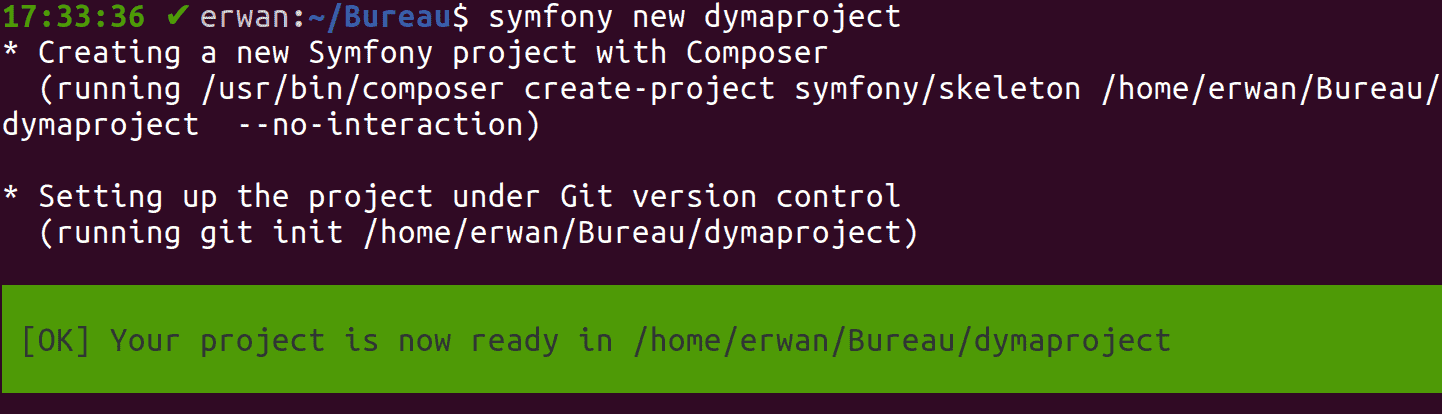
\includegraphics[width=15cm]{images/image1.png}
\end{center}

Ouvrez ensuite le projet dans {\tt Visual Studio Code}.

\subsection{Git par défaut}
Par défaut, {\tt Symfony} utilise Git et crée un premier commit avec les fichiers initiaux. Vous pouvez le voir en faisant :

\begin{verbatim}
git log
\end{verbatim}

Vous aurez par exemple :
\begin{center}
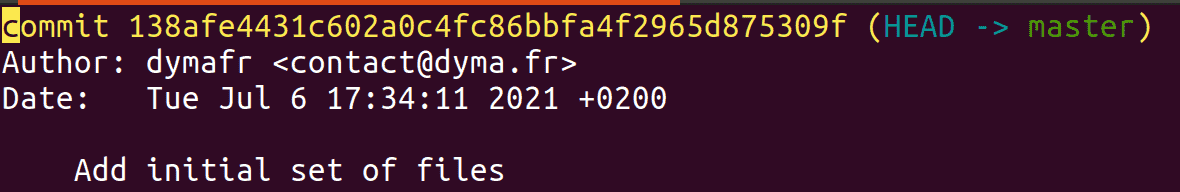
\includegraphics[width=15cm]{images/image2.png}
\end{center}

Lancer le serveur de développement. Pour lancer le serveur de développement local, il suffit d'ouvrir un terminal dans le dossier du projet et de faire :


\begin{verbatim}
symfony serve
\end{verbatim}
Le terminal vous indiquera l'adresse où votre application sera disponible localement :
\begin{center}

\includegraphics[width=15cm]{images/image3.png}
\end{center}

Vous pouvez couper le serveur à tout moment en faisant {\tt Ctrl + C}.

\subsection{Le fichier {\tt composer.json}}
Le fichier {\tt composer.json} contient toutes les dépendances du projet. Par défaut, {\tt Symfony} en installe plusieurs que nous allons voir ensemble.

\begin{itemize}

\item {\tt symfony/console }: permet de créer des interfaces en ligne de commande plus facilement. C'est le composant utilisé par le CLI Symfony.

\item {\tt symfony/dotenv} : permet d'automatiquement parser les fichiers avec l'extension .env pour charger les variables d'environnement et les rendre disponibles sur {\tt \$\_SERVER} ou {\tt \$\_ENV}.

\item {\tt symfony/flex} : permet de gérer l'architecture des dossiers et fichiers des projets Symfony. Il est utilisé notamment pour générer l'architecture de base lorsque nous avons fait symfony new. Il permet également d'installer de nouvelles dépendances.

\item {\tt symfony/framework-bundle} : librairie qui permet d'intégrer les composants {\tt Symfony} avec le {\tt framework}. Nous verrons que nous utiliserons de nombreux composants.

\item {\tt symfony/runtime} : gère le lancement de {\tt Symfony} quel que soit l'environnement ({\tt PHP-FPM, ReactPHP}, Swoole etc).

\item {\tt symfony/yaml} : permet de parser des fichiers contenant du {\tt YAML} et de les convertir en tableaux associatifs {\tt PHP}.
\end{itemize}


\subsection{Le fichier {\tt .gitignore}}
Nous ne passerons pas trop de temps sur {\tt Git}, nous vous invitons à faire la formation {\tt Git} disponible.

Ce fichier est déjà configuré pour les projets {\tt Symfony} pour ignorer les bons dossiers et fichiers lors des {\tt commit}s.

\subsection{Le fichier .env}
Le fichier .env contient les variables d'environnement.

Ce sont des variables contenant des valeurs nécessaires à l'application pour fonctionne (par exemple des mots de passe ou des secrets pour se connecter à des API tierces etc).

\subsection{Le dossier vendor}
Ce dossier contient toutes les dépendances installées et leurs dépendances en fonction du fichier {\tt composer.json}.

\subsection{Le dossier var}
\begin{itemize}
\item Le dossier {\tt var/cache} contient le système de cache de Symfony. Toute la configuration de l'application est parsée une seule fois et ensuite mise en cache dans ce dossier après le lancement. Cela permet de gagner en performance.

\item Le dossier {\tt var/logs} contient les logs de l'application. Ce sont des fichiers contenant toutes les informations sur les requêtes et les éventuelles erreurs. C'est très utile pour le débogage.
\end{itemize}
\subsection{Le dossier src}
Le dossier {\tt src} pour source contient le code de votre application. Par défaut, il contient la classe {\tt Kernel} (noyau) dans le fichier {\tt Kernel.php}. C'est le point d'entrée dans l'application : il va charger toutes les configurations de l'application.

\subsection{Le dossier public}
Le dossier {\tt public} contient tous les ressources statiques ou {\tt assets} (images, vidéos etc) et le point d'entrée {\tt index.php}.

\subsection{Le dossier config}
\begin{itemize}
\item Le dossier {\tt config} contient la configuration de l'application.

\item Le fichier {\tt routes.yaml} permet de configurer des routes.

\item Le fichier {\tt services.php} contient la configuration des services. Nous étudierons bien sûr les services en détail.

\item Le fichier {\tt bundles.php} permet d'activer ou de désactiver des packages. Les packages ou bundles sont des fonctionnalités utilisables directement dans l'application (c'est équivalent aux modules dans d'autres frameworks).\textbf{•}
\end{itemize}


\subsection{Le dossier bin}
Le dossier bin (pour binaries) contient les fichiers exécutables.


\section{Les composants Symfony}
Les composants Symfony sont des librairies PHP utilisables dans tout environnement PHP (donc pas forcément qu'avec Symfony).

Ces composants sont utilisés dans de très nombreux frameworks et projets PHP. Quelques exemples : bien sûr Symfony, PrestaShop, Drupal,

Nous allons prendre quelques exemples :
\begin{itemize}
\item {\tt Validator} : composant permettant de valider facilement les classes PHP.

\item {\tt Uid} : permet de gérer les identifiants uniques (UUIDs).

\item {\tt Serializer} : permet de transformer des entités dans un format spécifique (JSON ou YAML par exemple) et de désérialiser depuis ces formats vers des entités PHP.

HttpClient, HttpKernel et HttpFoundation : composants pour gérer les requêtes HTTP entrantes et les réponses HTTP sortantes.

\item {\tt Form} : permet de créer et de gérer des formulaires de manière simplifiée.

\end{itemize}

Il y a en tout une soixantaine de composants maintenus par l'équipe Symfony. Nous les verrons au fur et à mesure de nos besoins dans la formation.

\section{Les bundles Symfony}
Les bundles, contrairement aux composants, ne sont utilisables que dans le framework Symfony. Ils sont soit créés et maintenus par l'équipe Symfony, soit par des entités tiers. Ils sont alors appelés des bundles tiers (third-party bundles).

Un bundle permet d'ajouter une fonctionnalité à votre application. Symfony appelle les bundles également des packages, comme nous l'avons vu dans la leçon précédente.

Dans d'autres frameworks, les bundles sont appelés modules ou plugins. Prenons également quelques exemples :

\begin{itemize}
\item {\tt symfony/twig-bundle} : permet d'utiliser Twig de manière optimale avec Symfony. Twig est le moteur de templates pour créer les vues utilisé avec Symfony.

\item {\tt doctrine/doctrine-bundle} : même chose pour Doctrine. Doctrine est un ORM (couche d'abstraction à la base de données) pour PHP.

\item {\tt symfony/swiftmailer-bundle} : permet de gérer les envois d'emails avec les principaux services (Mandrill, SendGrid, Amazon SES etc).

\end{itemize}
Il y a bien sûr beaucoup d'autres bundles Symfony que nous utiliserons au fur et à mesure.

\section{Fonctionnement d'une application Symfony}
Nous allons brièvement voir dans l'ordre les éléments qui gèrent une requête HTTP entrante d'un client :
\begin{center}
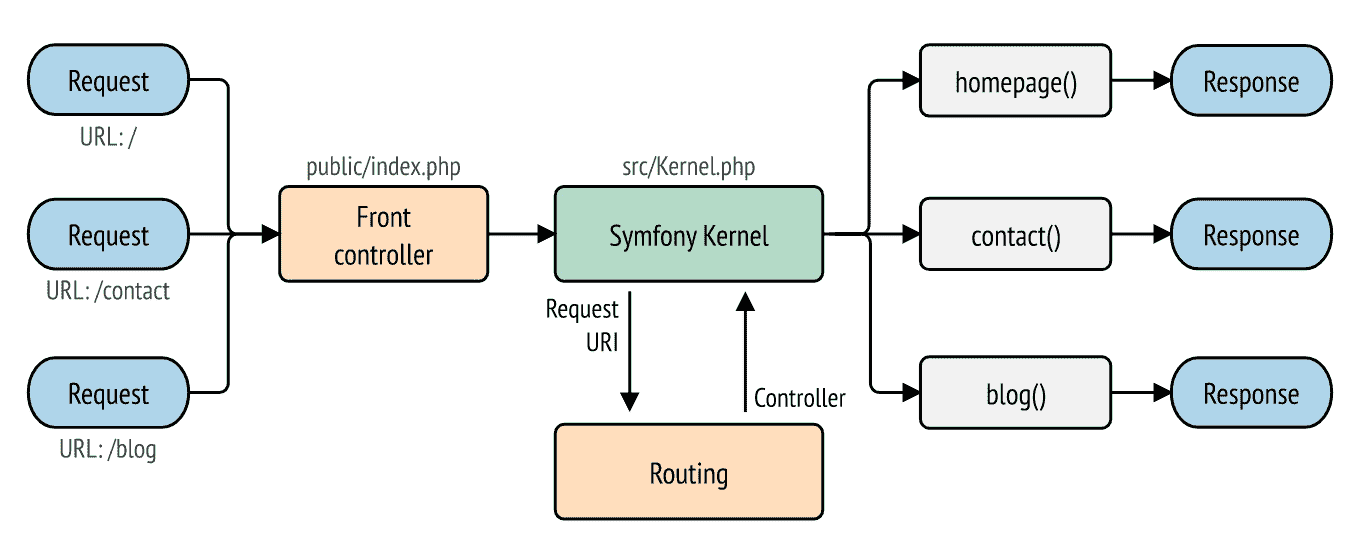
\includegraphics[width=15cm]{images/image4.png}
\end{center}

\subsection{Le script index.php}
Lorsqu'une requête HTTP est reçue par le serveur Web (par exemple NGINX) puis transmise à PHP-FPM (grâce au protocole FastCGI), le premier script PHP à être exécuté est {\tt public/index.php}. On l'appelle point d'entrée ou Front controller.

Le front controller est le contrôleur qui gère l'ensemble des requêtes d'une application. Autrement dit, toutes les requêtes HTTP entraînent obligatoirement l'exécution de ce script.

Si vous avez suivi le cours PHP vous noterez que c'est déjà une différence avec une application PHP basique qui exécute un script différent suivant la requête HTTP et qui n'a donc pas un seul point d'entrée pour l'ensemble des requêtes.

Voici son contenu :
\begin{minted}[
mathescape,
framesep=2mm,
baselinestretch=1.2,
fontsize=\footnotesize,
linenos
]{php}
<?php

use App\Kernel;

require_once dirname(__DIR__).'/vendor/autoload_runtime.php';

return function (array $context) {
    return new Kernel($context['APP_ENV'], (bool) $context['APP_DEBUG']);
};
\end{minted}




Ce script commence par initialiser la fonctionnalité du chargement automatique en fonction de l'environnement (autoload).

Ce script crée ensuite une instance de la classe Kernel.

\subsection{La classe Kernel}
La classe Kernel est chargée par le script index.php, elle se trouve dans src/kernel.php.

Voici son contenu :
\begin{minted}[
mathescape,
framesep=2mm,
baselinestretch=1.2,
fontsize=\footnotesize,
linenos
]{php}
<?php

namespace App;

use SymfonyBundleFrameworkBundleKernelMicroKernelTrait;
use SymfonyComponentHttpKernelKernel as BaseKernel;

class Kernel extends BaseKernel
{
    use MicroKernelTrait;
}
\end{minted}

{\tt Symfony\\Component\\HttpKernel\\Kernel} qui est ici renommée en {\tt BaseKernel} est le cœur de Symfony. Elle va initialiser tous les {\tt bundles Symfony} avec la configuration de votre application.

Vous pouvez aller regarder les fonctions d'initialisation des bundles dans {\tt dymaproject/vendor/symfony/http-kernel/Kernel.php}

Vous y trouverez notamment une fonction initializeBundles() qui est chargée de cette initialisation.

\subsection{La fonction handle()}
Une fois toutes les configurations, le routing et les bundles chargés, la requête est gérée par la fonction {\tt handle()} de la classe {\tt HttpKernel}.

Cette fonction a pour objectif de partir d'une requête HTTP et de la transformer en la réponse HTTP attendue.

C'est donc une fonction très importante dont le schéma suivant résume son fonctionnement :
\begin{center}
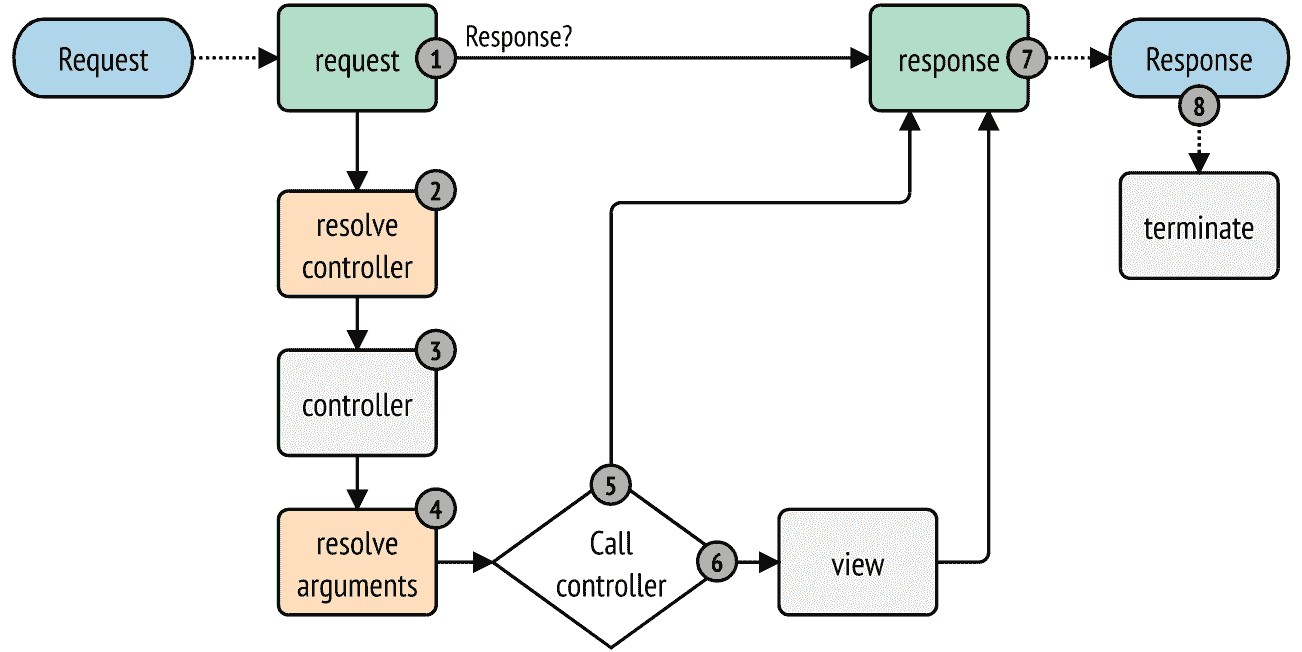
\includegraphics[width=15cm]{images/image5.png}
\end{center}

Cette fonction va envoyer des événements qui sont ensuite gérés par des gestionnaires d'événements.

Nous allons voir les grandes étapes du processus :

\begin{enumerate}
\item Un événement kernel.request est émis. Plusieurs gestionnaires sont appelés à ce niveau. Par exemple, le gestionnaire du bundle Security qui va déterminer si la requête est autorisée ou non. La requête peut être transformée en réponse 403 (pour forbidden) et retournée à ce moment. Un autre gestionnaire important pour cet événement est le Router, il va déterminer quel contrôleur doit être appelé en fonction de la requête.

\item  Le Contrôleur est résolu. La fonction handle() va appeler une fonction getController() (située dans {\tt dymaproject/vendor/symfony/http-kernel/Controller/ControllerResolver.php}) qui va être chargé de récupérer et d'exécuter le bon contrôleur en fonction de la propriété \_controller qui a été placé par le Router sur le tableau associatif Request.

Vous pouvez voir cette mécanique au début de la fonction getController() :
\begin{minted}[
mathescape,
framesep=2mm,
baselinestretch=1.2,
fontsize=\footnotesize,
linenos
]{php}
<?php
public function getController(Request $request) {
  if (!$controller = $request->attributes->get('_controller')) {
    if (null !== $this->logger) {
      $this->logger->warning('Unable to look for the controller as the "_controller" parameter is missing.');
    }
    return false;
  }
}
\end{minted}
\item  Un événement kernel.controller est émis. Il permet d'exécuter des gestionnaires d'événement juste avant que le contrôleur récupéré ne soit exécuté. C'est un design pattern commun appelé hooks en programmation. Cela permet d'exécuter du code lors d'événements clés.

\item  Récupération des arguments pour le contrôleur. Avant l'exécution du contrôleur, une fonction getArguments() va récupérer les arguments à passer au contrôleur en fonction de l'environnement et de la configuration.

\item  Exécution du contrôleur. Le contrôleur, qui est chargé de construire la réponse à renvoyer au client, est exécuté. Il va créer une réponse qui peut être une page HTML, une réponse au format JSON ou toute autre réponse HTTP valide. C'est à cette étape que sera exécuté votre code : votre contrôleur, qui va éventuellement appeler vos modèles et vos vues.

\item  Un événement {\tt kernel.view} est émis. Permet de gérer les cas où aucune réponse n'est retournée par le contrôleur. Par défaut, Symfony n'a aucune gestionnaire pour cet événement et vos contrôleurs doivent obligatoirement retourner une réponse. Certains bundles utilisent cet événement, comme par exemple {\tt FOSRestBundle}.

\item  Un événement {\tt kernel.response} est émis. Permet d'exécuter des gestionnaires juste avant que la réponse ne soit envoyée au client. Des exemples d'utilisation sont la modification des headers de la réponse, l'ajout de cookies etc.

\item  Un événement {\tt kernel.terminate} est émis. La réponse a été envoyée au client. Cet événement permet de procéder aux nettoyages ou à des tâches pouvant être réalisées après la réponse HTTP (par exemple, enregistrement de données d'analyse, envoi d'emails etc).
\end{enumerate}


\section{Création d'une première page}
\subsection{Utiliser HTTPS en local}
Lorsque vous exécutez symfony serve, vous aurez l'avertissement suivant :
\begin{center}
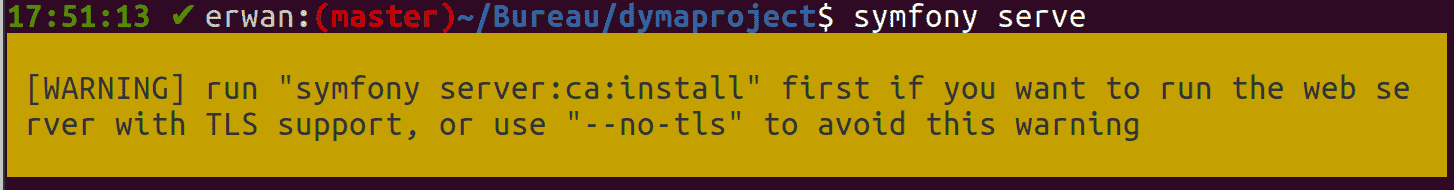
\includegraphics[width=15cm]{images/image6.png}
\end{center}

Il signifie que par défaut, votre serveur de développement local utilisera le protocole HTTP et non sa version sécurisée, le protocole {\tt HTTPS} (utilisant le protocole {\tt TLS}).

Ouvrez donc un terminal dans votre projet et entrez :
\begin{verbatim}
symfony server:ca:install
\end{verbatim}

Le {\tt CLI Symfony} créera un certificat local pour pouvoir utiliser localement {\tt HTTPS}. Il l'ajoutera à vos navigateurs automatiquement :
\begin{verbatim}
The local CA is now installed in the system trust store!
The local CA is now installed in the Firefox and/or Chrome/Chromium trust store (requires browser restart)!
\end{verbatim}

Il faudra les redémarrer pour que le certificat soit pris en compte. Ce certificat n'est évidemment valide que lors du développement en local. Vous pouvez ensuite relancer votre serveur de développement :

\begin{verbatim}
symfony serve
\end{verbatim}

Il sera cette fois disponible par défaut à l'adresse {\tt https://127.0.0.1:8000/}.

Notez bien l'utilisation du protocole {\tt HTTPS} dans {\tt l'URL}.

\subsection{Le langage {\tt YAML}}
Le {\tt YAML} (pour YAML Ain't Markup Language ou "YAML n'est pas un langage de balisage") est un langage permettant de représenter des informations élaborées tout en conservant une grande lisibilité. Il repose principalement sur l'indentation.

C'est un langage utilisé le plus souvent pour des fichiers de configuration.

Nous allons voir les principaux éléments de la syntaxe de ce langage car tout ce que nous verrons à partir de maintenant utilisera du {\tt YAML} :

\# permet de commenter une ligne s'il est placé au début d'une ligne. S'il est avant une chaîne de caractère, il signifie nombre littéral.

$\sim$ signifie valeur nulle.

$-$ permet de créer des listes. Chaque élément d'une liste doit être précédé par - puis un espace. Il doit y avoir un élément par ligne.

clé: valeur permet de déclarer un map clé / valeur.

L'indentation par des espaces permet de créer une hiérarchie, par exemple :

\begin{minted}[
mathescape,
framesep=2mm,
baselinestretch=1.2,
fontsize=\footnotesize,
linenos
]{yaml}
paul:
  nom: Paul Dupont
  emploi: Developer
\end{minted}

Une structure plus complexe :
\begin{minted}[
mathescape,
framesep=2mm,
baselinestretch=1.2,
fontsize=\footnotesize,
linenos
]{yaml}
- paul:
    nom: Paul Dupont
    emploi: Developer
    languages:
      - javascript
      - css
      - html
      - php
\end{minted}

\subsection{Le fichier {\tt config/routes/routes.yaml}}
Dans {\tt Symfony}, vous pouvez écrire des routes directement dans les contrôleurs, comme nous le verrons, ou dans des fichiers {\tt YAML}, {\tt XML} ou {\tt PHP}.

Depuis {\tt Symfony 5.1} seules les routes dans des fichiers écrits en {\tt YAML} sont chargées par défaut. Nous ne verrons donc pas les routes écrites en XML et PHP qui ne sont plus recommandées.

Par défaut, le fichier de route chargé est {\tt config/routes/routes.yaml} :
\begin{minted}[
mathescape,
framesep=2mm,
baselinestretch=1.2,
fontsize=\footnotesize,
linenos
]{yaml}
controllers:
    resource:
        path: ../src/Controller/
        namespace: App\Controller
    type: attribute
\end{minted}

\begin{itemize}
\item {\tt controllers} indique le début de la configuration des contrôleurs.

\item {\tt resource} est utilisée pour déterminer la source des contrôleurs, c'est-à-dire où les fichiers contenant les contrôleurs sont situés.

path spécifie le chemin du répertoire où les fichiers des contrôleurs sont situés. Dans ce cas, les contrôleurs sont stockés dans le dossier Controller du répertoire src.

\item {\tt namespace} spécifie le namespace PHP des contrôleurs. Les namespaces PHP sont utilisés pour organiser et regrouper les classes de manière logique, évitant ainsi les conflits de noms entre les classes. Ici, le namespace des contrôleurs est {\tt App\\Controller}.

\item {\tt type: attribute} indique que les contrôleurs sont définis en utilisant des attributs PHP (disponibles à partir de PHP 8.0). Les attributs permettent d'ajouter des métadonnées à une classe, une méthode ou une propriété. Dans le contexte de Symfony, les attributs sont utilisés pour définir des informations sur le routage, telles que l'URL d'une route et la méthode HTTP associée.

\end{itemize}

Modifiez le fichier {\tt config/routes/routes.yaml} pour ajouter une route pour notre premier contrôleur :
\begin{minted}[
mathescape,
framesep=2mm,
baselinestretch=1.2,
fontsize=\footnotesize,
linenos
]{yaml}
controllers:
    resource:
        path: ../src/Controller/
        namespace: App\Controller
    type: attribute

index:
  path: /
  controller: App\Controller\DefaultController::index
\end{minted}

\begin{itemize}
\item {\tt index} est le nom de la route.

\item {\tt path} est le chemin de la route qui va matcher avec l'URI de la requête HTTP.

\item {\tt controller} est le chemin vers le contrôleur et l'action à exécuter pour la route. Par exemple ici, la classe contrôleur à exécuter est DefaultController, qui se situe dans dymaproject/src/Controller. L'action est située après les doubles deux points ::. Elle correspond à la méthode sur la classe contrôleur qui va être exécutée à chaque requête qui correspond à la route.
\end{itemize}

\subsection{Création du contrôleur}
Pour le moment, le contrôleur n'existe pas et vous aurez une page d'erreur lorsque vous irez sur {\tt https://127.0.0.1:8000/}.

\begin{center}
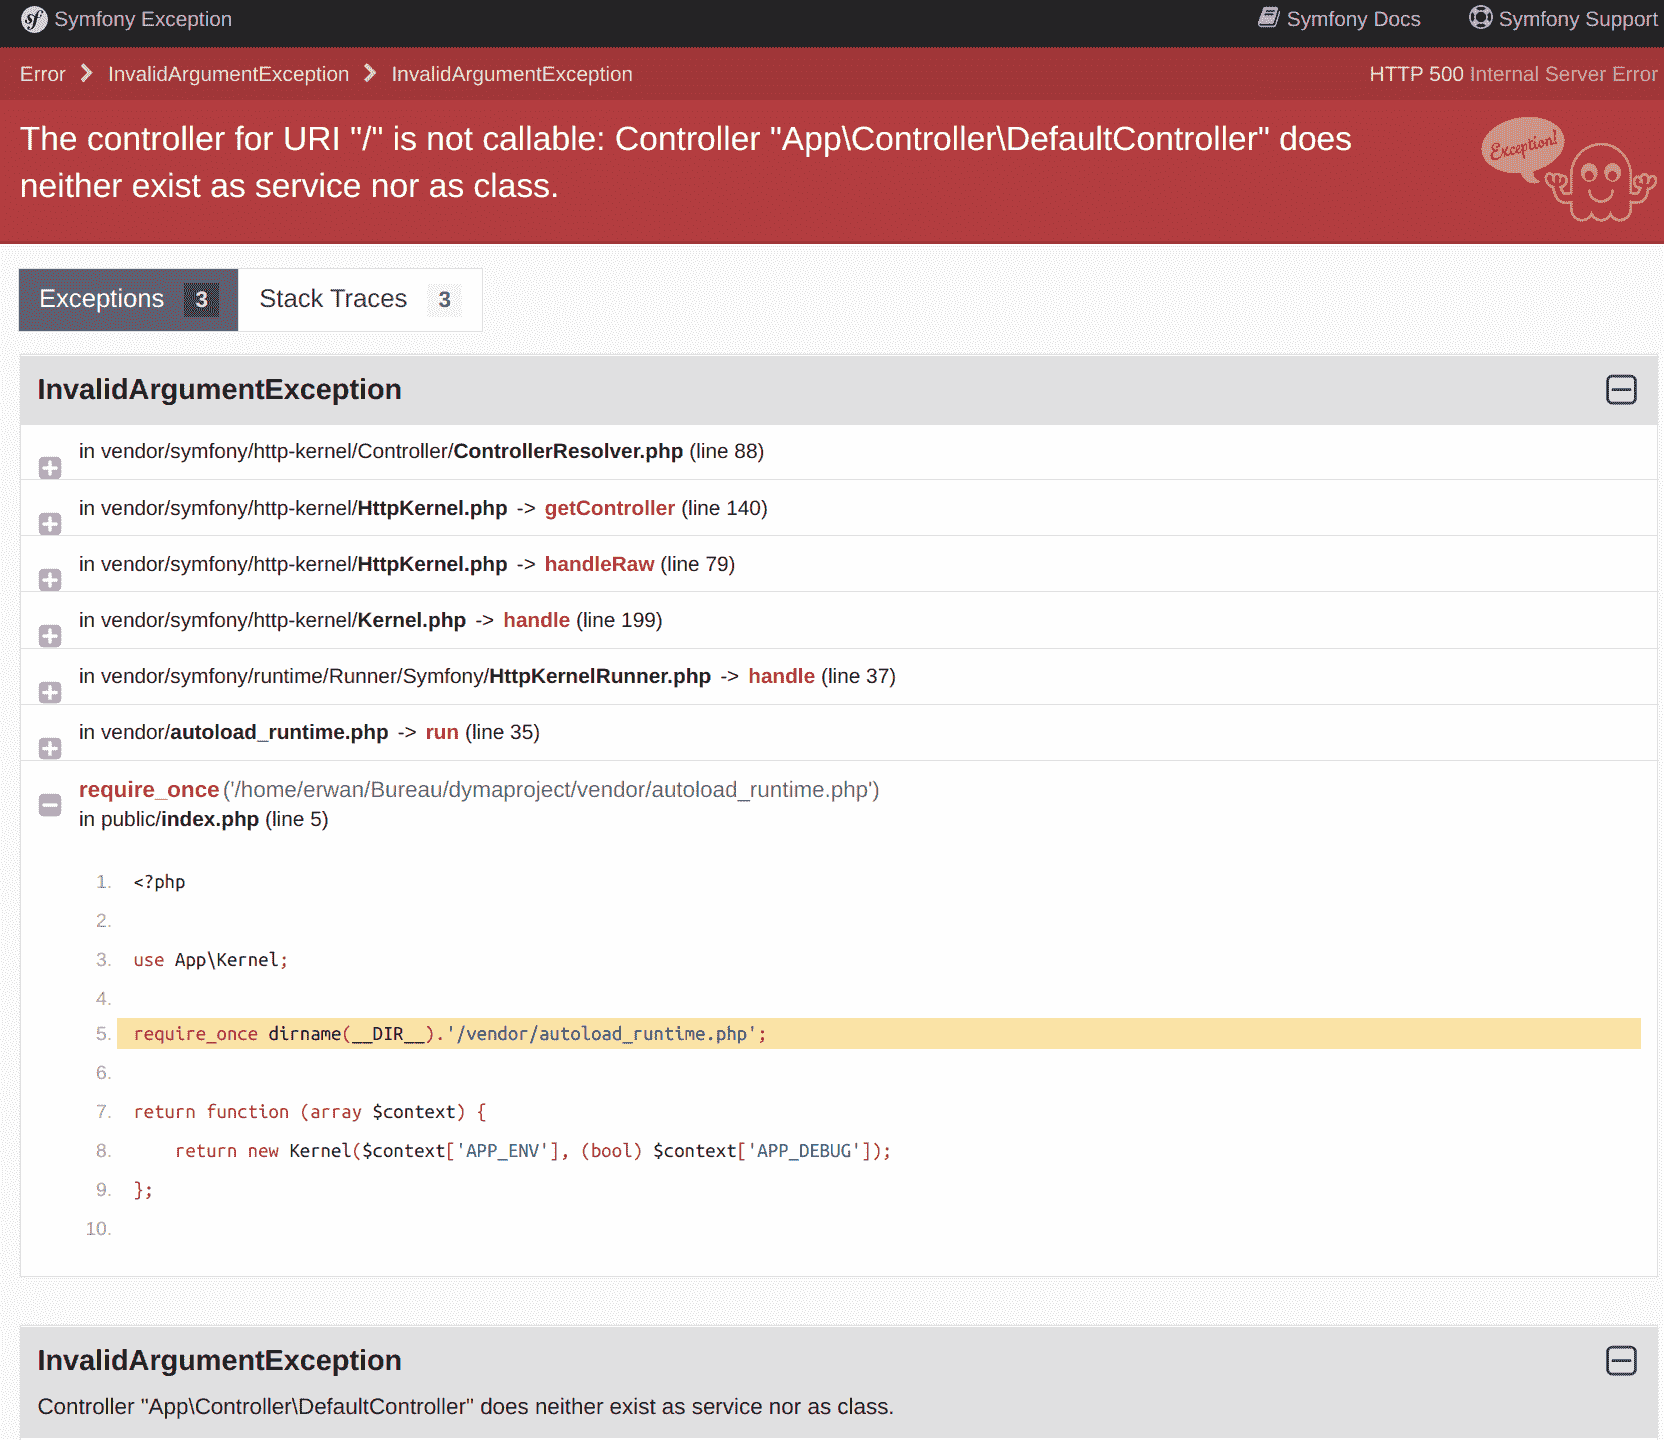
\includegraphics[width=15cm]{images/image7.png}
\end{center}

Notez l'erreur : "Le contrôleur {\tt DefaultController} n'existe pas".

Nous devons donc le créer dans {\tt src/Controller/DefaultController.php} :

\begin{minted}[
mathescape,
framesep=2mm,
baselinestretch=1.2,
fontsize=\footnotesize,
linenos
]{php}
<?php

namespace App\Controller;

use Symfony\Component\HttpFoundation\Response;

class DefaultController
{
  public function index()
  {
    return new Response('<h1>Hello World !</h1>');
  }
}
\end{minted}

Expliquons en détail ce contrôleur.

{\tt namespace App\\Controller;} : permet à la classe d'être importée automatiquement par l'{\tt autoload}. Il faut impérativement commencer par {\tt App} puis respecter le chemin depuis src jusqu'à la classe. Comme notre classe est dans le dossier {\tt src/Controller} il faut donc indiquer {\tt App\\Controller}.

Si vous voulez en savoir plus revoyez les chapitres namespace et Composer et autoload dans la formation PHP.

Nous devons ensuite déclarer la classe en respectant le nom donné dans la route sur la propriété {\tt controller}. Dans notre cas, il faut donc obligatoirement appeler la classe {\tt DefaultController}.

Il faut ensuite créer une méthode sur la classe qui correspond au nom de l'action déclarée sur la route. Dans notre cas l'action est index. Nous devons donc créer une méthode {\tt index()} qui sera exécutée.

Dans cette méthode, nous devons obligatoirement retourner une réponse. Comme nous l'avons vu, l'objectif d'un contrôleur est de recevoir une requête HTTP et de retourner une réponse HTTP.

Pour créer un objet {\tt Response}, commencez à taper {\tt Resp} et vous aurez l'autocomplétion et l'auto-importation de la classe par {\tt VS Code}.


\section{L'objet {\tt Request} du composant {\tt HttpFoundation}}
\subsection{Le composant {\tt HttpFoundation}}
En {\tt PHP}, vous savez qu'il existe un ensemble de variables globales. Par exemple : {\tt \$\_SERVER}, {\tt \$\_GET} ou {\tt \$\_COOKIE}. Le composant {\tt Symfony HttpFoundation} permet de remplacer ces variables globales par des objets, et notamment par {\tt Request} et {\tt Response}.

\subsection{L'objet {\tt Request}}
Pour créer un objet {\tt Request}, il suffit de faire :
\begin{minted}[
mathescape,
framesep=2mm,
baselinestretch=1.2,
fontsize=\footnotesize,
linenos
]{php}
<?php
use Symfony\Component\HttpFoundation\Request;

$request = Request::createFromGlobals();
\end{minted}

La méthode statique {\tt createFromGlobals()} permet de créer l'objet en passant la plupart des variables globales PHP à une méthode {\tt createRequestFromFactory()} :
\begin{minted}[
mathescape,
framesep=2mm,
baselinestretch=1.2,
fontsize=\footnotesize,
linenos
]{php}
public static function createFromGlobals()
{
  $request = self::createRequestFromFactory($_GET, $_POST, [], $_COOKIE, $_FILES, $_SERVER);

  if (0 === strpos($request->headers->get('CONTENT_TYPE', ''), 'application/x-www-form-urlencoded')
    && \in_array(strtoupper($request->server->get('REQUEST_METHOD', 'GET')), ['PUT', 'DELETE', 'PATCH'])
  ) {
    parse_str($request->getContent(), $data);
    $request->request = new InputBag($data);
  }

  return $request;
}
\end{minted}

Sur l'objet {\tt Request}, nous retrouvons les propriétés suivantes :

\begin{itemize}
\item {\tt request} qui contient les informations de la variable globale {\tt \$\_POST}.

\item {\tt query} qui contient les informations de la variable globale {\tt \$\_GET}.

\item {\tt cookies} qui contient les informations de la variable globale {\tt \$\_COOKIE}.

\item {\tt attributes} qui contient des propriétés propres à l'application.

\item {\tt files} qui contient les informations de la variable globale {\tt \$\_FILES}.

\item {\tt server} qui contient les informations de la variable globale {\tt \$\_SERVER}.

\item {\tt headers} qui contient les informations sur les en-têtes qui se trouvent pour la plupart sur la variable globale {\tt \$\_SERVER}.
\end{itemize}
Tous ces objets sont des instances des classes {\tt ParameterBag,InputBag, FileBag, ServerBag} ou {\tt HeaderBag}.

Ces classes contiennent des méthodes permettant d'accéder aux propriétés et de les modifier. Nous verrons toutes ces méthodes en détail au cours de la formation.

Pour donner un exemple, si nous avons une requête {\tt HTTP GET} avec une {\tt query string}, par exemple {\tt ?name=paul} :

\begin{minted}[
mathescape,
framesep=2mm,
baselinestretch=1.2,
fontsize=\footnotesize,
linenos
]{php}
<?php

$request->query->get('name');
\end{minted}
Permet d'accéder à la valeur de la {\tt query string name} et donc ici de retourner {\tt paul}.

\subsection{Code de la vidéo}
Créer un nouveau dossier {\tt php}. Dans ce dossier, {\tt installez symfony/var-dumper} et {\tt symfony/http-foundation} :
\begin{verbatim}
composer require symfony/http-foundation symfony/var-dumper
\end{verbatim}

Créez un fichier {\tt index.php} :

\begin{minted}[
mathescape,
framesep=2mm,
baselinestretch=1.2,
fontsize=\footnotesize,
linenos
]{php}
<?php

use Symfony\Component\HttpFoundation\Request;

require __DIR__ . '/vendor/autoload.php';

$request = Request::createFromGlobals();

dump($request);
dd($request->query->get('name'));
\end{minted}
Lancez ensuite le serveur de développement :
\begin{verbatim}
php -S localhost:3000
\end{verbatim}

Rendez-vous sur {\tt http://localhost:3000/}.



\section{L'objet {\tt Response} du composant {\tt HttpFoundation}}
\subsection{L'objet {\tt Response}}
L'objet {\tt Response} permet de créer, modifier et envoyer une réponse {\tt HTTP}.

\subsubsection{Créer une Response}
Étudions son constructeur :

\begin{minted}[
mathescape,
framesep=2mm,
baselinestretch=1.2,
fontsize=\footnotesize,
linenos
]{php}
<?php

public function __construct(?string $content = '', int $status = 200, array $headers = [])
{
  $this->headers = new ResponseHeaderBag($headers);
  $this->setContent($content);
  $this->setStatusCode($status);
  $this->setProtocolVersion('1.0');
}
\end{minted}
Remarquez que tous les arguments sont optionnels et qu'ils ont des valeurs par défaut.
\begin{itemize}
\item Le premier argument est le contenu de la réponse {\tt HTTP}, qui est vide par défaut.
\item Le second argument est le statut de la réponse {\tt HTTP}, qui {\tt 200} pour {\tt OK} par défaut.
\item Le troisième argument est un tableau associatif pour les en-têtes, qui est vide par défaut.

\end{itemize}

Pour créer une réponse vous pouvez donc par exemple faire :

\begin{minted}[
mathescape,
framesep=2mm,
baselinestretch=1.2,
fontsize=\footnotesize,
linenos
]{php}
<?php

$response = new Response(
  'Vous n\’êtes pas autorisé à voir cette page',
  Response::HTTP_FORBIDDEN,
  ['content-type' => 'text/html']
);
\end{minted}

Remarquez que nous utilisons une constante pour le statut, tous les codes de statut sont disponibles sur la classe {\tt Response} :

\begin{minted}[
mathescape,
framesep=2mm,
baselinestretch=1.2,
fontsize=\footnotesize,
linenos
]{php}
<?php
  public const HTTP_CONTINUE = 100;
  public const HTTP_SWITCHING_PROTOCOLS = 101;
  public const HTTP_PROCESSING = 102;            // RFC2518
  public const HTTP_EARLY_HINTS = 103;           // RFC8297
  public const HTTP_OK = 200;
  public const HTTP_CREATED = 201;
  public const HTTP_ACCEPTED = 202;
  public const HTTP_NON_AUTHORITATIVE_INFORMATION = 203;
  public const HTTP_NO_CONTENT = 204;
  public const HTTP_RESET_CONTENT = 205;
  public const HTTP_PARTIAL_CONTENT = 206;
  public const HTTP_MULTI_STATUS = 207;          // RFC4918
  public const HTTP_ALREADY_REPORTED = 208;      // RFC5842
  public const HTTP_IM_USED = 226;               // RFC3229
  public const HTTP_MULTIPLE_CHOICES = 300;
  public const HTTP_MOVED_PERMANENTLY = 301;
  public const HTTP_FOUND = 302;
  public const HTTP_SEE_OTHER = 303;
  public const HTTP_NOT_MODIFIED = 304;
  public const HTTP_USE_PROXY = 305;
  public const HTTP_RESERVED = 306;
  public const HTTP_TEMPORARY_REDIRECT = 307;
  public const HTTP_PERMANENTLY_REDIRECT = 308;  // RFC7238
  public const HTTP_BAD_REQUEST = 400;
  public const HTTP_UNAUTHORIZED = 401;
  public const HTTP_PAYMENT_REQUIRED = 402;
  public const HTTP_FORBIDDEN = 403;
  public const HTTP_NOT_FOUND = 404;
  public const HTTP_METHOD_NOT_ALLOWED = 405;
  public const HTTP_NOT_ACCEPTABLE = 406;
  public const HTTP_PROXY_AUTHENTICATION_REQUIRED = 407;
  public const HTTP_REQUEST_TIMEOUT = 408;
  public const HTTP_CONFLICT = 409;
  public const HTTP_GONE = 410;
  public const HTTP_LENGTH_REQUIRED = 411;
  public const HTTP_PRECONDITION_FAILED = 412;
  public const HTTP_REQUEST_ENTITY_TOO_LARGE = 413;
  public const HTTP_REQUEST_URI_TOO_LONG = 414;
  public const HTTP_UNSUPPORTED_MEDIA_TYPE = 415;
  public const HTTP_REQUESTED_RANGE_NOT_SATISFIABLE = 416;
  public const HTTP_EXPECTATION_FAILED = 417;
  public const HTTP_I_AM_A_TEAPOT = 418;                                               // RFC2324
  public const HTTP_MISDIRECTED_REQUEST = 421;                                         // RFC7540
  public const HTTP_UNPROCESSABLE_ENTITY = 422;                                        // RFC4918
  public const HTTP_LOCKED = 423;                                                      // RFC4918
  public const HTTP_FAILED_DEPENDENCY = 424;                                           // RFC4918
  public const HTTP_TOO_EARLY = 425;                                                   // RFC-ietf-httpbis-replay-04
  public const HTTP_UPGRADE_REQUIRED = 426;                                            // RFC2817
  public const HTTP_PRECONDITION_REQUIRED = 428;                                       // RFC6585
  public const HTTP_TOO_MANY_REQUESTS = 429;                                           // RFC6585
  public const HTTP_REQUEST_HEADER_FIELDS_TOO_LARGE = 431;                             // RFC6585
  public const HTTP_UNAVAILABLE_FOR_LEGAL_REASONS = 451;
  public const HTTP_INTERNAL_SERVER_ERROR = 500;
  public const HTTP_NOT_IMPLEMENTED = 501;
  public const HTTP_BAD_GATEWAY = 502;
  public const HTTP_SERVICE_UNAVAILABLE = 503;
  public const HTTP_GATEWAY_TIMEOUT = 504;
  public const HTTP_VERSION_NOT_SUPPORTED = 505;
  public const HTTP_VARIANT_ALSO_NEGOTIATES_EXPERIMENTAL = 506;                        // RFC2295
  public const HTTP_INSUFFICIENT_STORAGE = 507;                                        // RFC4918
  public const HTTP_LOOP_DETECTED = 508;                                               // RFC5842
  public const HTTP_NOT_EXTENDED = 510;                                                // RFC2774
  public const HTTP_NETWORK_AUTHENTICATION_REQUIRED = 511;
\end{minted}

Cela permet une meilleure lisibilité du code et de ne pas se tromper sur le statut.

\subsubsection{Modifier une {\tt Response}}
La classe possède également des propriétés publiques qui sont modifiables avec des setters.

{\bf Il est ainsi possible de modifier un objet Response une fois que celui-ci a été créé}.

Pour rappel, un setter est une méthode permettant de modifier une propriété sur un objet.

Par exemple, pour modifier le contenu de la réponse :

\begin{minted}[
mathescape,
framesep=2mm,
baselinestretch=1.2,
fontsize=\footnotesize,
linenos
]{php}
<?php
$response->setContent('Hello World !');
\end{minted}

Même chose pour les en-têtes :

\begin{minted}[
mathescape,
framesep=2mm,
baselinestretch=1.2,
fontsize=\footnotesize,
linenos
]{php}
<?php
$response->headers->set('Content-Type', 'text/plain');
\end{minted}
Et pour le code de statut :

\begin{minted}[
mathescape,
framesep=2mm,
baselinestretch=1.2,
fontsize=\footnotesize,
linenos
]{php}
<?php
$response->setStatusCode(Response::HTTP_NOT_FOUND);
\end{minted} 

\subsubsection{Envoyer la Response}
Une fois que l'objet Response est prêt à être envoyé au client, il suffit d'appeler la méthode send() :

\begin{minted}[
mathescape,
framesep=2mm,
baselinestretch=1.2,
fontsize=\footnotesize,
linenos
]{php}
<?php
$response->send();
\end{minted} 

\subsection{Les réponses au format {\tt JSON}}
Bien qu'il soit possible d'utiliser l'objet {\tt Response} pour envoyer une réponse au format {\tt JSON}, ce n'est pas pratique car il faut manuellement définir l'entête {\tt Content-Type} et encoder l'entité {\tt PHP} au format {\tt JSON}.

Le composant {\tt HttpFoundation} a donc une classe spécifique qui permet de faire cela automatiquement pour vous : {\tt JsonResponse}.

Vous pouvez ainsi directement faire :
\begin{minted}[
mathescape,
framesep=2mm,
baselinestretch=1.2,
fontsize=\footnotesize,
linenos
]{php}
<?php
use Symfony\Component\HttpFoundation\JsonResponse;

$response = new JsonResponse(['prenom' => 'Jean' ]);
\end{minted} 

\subsection{Code de la vidéo : dossier {\tt php}}
Dans le fichier {\tt index.php} mettez le code suivant :

\begin{minted}[
mathescape,
framesep=2mm,
baselinestretch=1.2,
fontsize=\footnotesize,
linenos
]{php}
<?php

use Symfony\Component\HttpFoundation\Response;

require __DIR__ . '/vendor/autoload.php';

$response = new Response('<h2>First !</h2><h1>Hello World ! </h1>');

$response->headers->set('salut', 'ca va');

$response->send();
\end{minted} 

Lancez ensuite le serveur de développement :
\begin{verbatim}
php -S localhost:3000
\end{verbatim}

Rendez-vous sur {\tt http://localhost:3000/}.

\subsection{Code de la vidéo : dossier {\tt dymaproject}}
De retour sur le projet {\tt Symfony}, nous modifions notre contrôleur pour récupérer l'objet Request créé par {\tt Symfony} dans l'action index :

\begin{minted}[
mathescape,
framesep=2mm,
baselinestretch=1.2,
fontsize=\footnotesize,
linenos
]{php}
<?php

namespace App\Controller;

use Symfony\Component\HttpFoundation\Request;
use Symfony\Component\HttpFoundation\Response;

class DefaultController
{
  public function index(Request $request)
  {
    dd($request);
    return new Response('<h1>Hello World !</h1>');
  }
}
\end{minted} 

{\tt Symfony} passe automatiquement l'objet {\tt Request}, qu'il créée automatiquement, en argument des actions.

Pour rappel, les actions sont les méthodes sur les classes des contrôleurs qui sont exécutées lorsqu'une requête {\tt HTTP} correspond à une route.

Notez bien la propriété {\tt attributes} sur l'objet requête :

\begin{center}
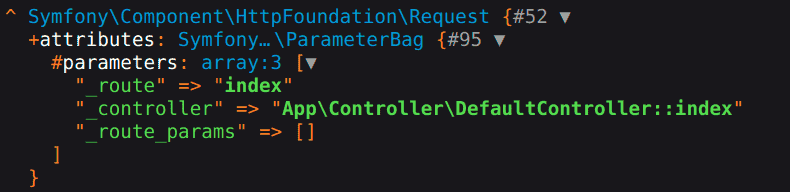
\includegraphics[width=15cm]{images/image8.png}
\end{center}

Comme nous l'avons vu, il s'agit d'une instance de la classe {\tt ParamaterBag} qui contient des paires clé / valeur créées par l'application.

Dans ces paires nous retrouvons, comme prévu, le nom de la route dans {\tt \_route} et le chemin vers le contrôleur, et plus précisément son action, à exécuter dans {\tt \_controler}.

\end{document}




